\documentclass[12pt,t]{beamer}
\usetheme{metropolis}
\usepackage{listings} % Pakke til kode
\usepackage{pslatex}        % pæn skrift
\usepackage[utf8]{inputenc} % Implementerer Unicode
\usepackage{algpseudocode}
\usepackage{algorithm}
\usepackage{marvosym}
\setbeamersize{description width=0.57cm}
\metroset{block=fill}
\title{IT fagene i de gymnasiale uddannelser}
\subtitle{Machine learning, datamining og big data}
\author{
        Benjamin Rotendahl
}

\date[]{\today}


\begin{document}

\frame{\titlepage}

\begin{frame}[c]{Benjamin Rotendahl}
    \begin{block}{Hvem er det?}
        \begin{itemize}
            \item Kæmpe nørd. \pause
            \item Datalogistuderende ved Københavns Univsersitet. \pause
            \item Frivilig/studentermedhjælper/bestyrelsesmedlem i  Coding
                  Pirates. \pause
            \item Medlem af Datalogisk Instituts gymnasietjeneste.
        \end{itemize}
    \end{block}
\end{frame}


\begin{frame}[c]{Programmet for idag}
        \begin{description}
            \item[\alert{Intro til Machine Learning}]~\\
            Forklaring af de overorddne ideer og tanker bag machine learning

            \pause
            \item[\alert{Perceptron algoritmen}]~\\
            En simpel machine learning algortime bygget på vektorregning.

            \pause
            \item[\alert{Fremvising og øvelser i iPythone}]~\\
            Interaktive øvelser i det fremragende iPython.

            \pause
            \item[\alert{Afrunding og spørgsmål}]~\\
        \end{description}
\end{frame}

 \section{Hvad er Machine Learning}

     \begin{frame}[t]{Hvad er Machine Learning}
         \begin{block}{Problemstilling}
             Vi indsamler større og større mængder af data hele tiden, så meget
             at det har fået sit eget buzzword \alert{Big Data}. \\
         \end{block}
         \pause
         \begin{block}{Løsning}
            Finde en måde at få computere til at finde de underliggende mønstre
            og bruge den viden/erfaring der ligger i data'en.
         \end{block}
         \pause
         \begin{block}{Hvornår er ML godt?}
             \begin{enumerate}
                 \item Der eksisterer et mønster \pause
                 \item Vi kan ikke finde en matematisk formel \pause
                 \item Vi har data på problemet
             \end{enumerate}
         \end{block}
     \end{frame}

    \begin{frame}[t]{Dagens øvelse}
        \begin{quote}
            Vi er blevet hyret af et hospital da de har hørt at vi IT-folk
            kan hjælpe deres patienter.
        \end{quote}
        \pause
        \begin{block}{Problemstilling}
            Vi skal lave et system der, givet data om en patient, kan bestemme
            om deres svulst er godartet eller ondartet.
        \end{block}
        \pause
        \centering Hmm, det var da et ret generelt problem $\dots$
        \pause
        \begin{block}{Problemstilling}
            Vi skal lave et system der, givet data om en \alert{kunde},
            kan bestemme om det er en god forretning at låne dem penge.
        \end{block}
        \pause
        \centering Problemet kaldes \textbf{klassificering}, gode løsninger kan
        have stor indflydelse inden for mange felter.
    \end{frame}

    \begin{frame}[t]{Eksempel}
        \begin{block}{Kan Machine Learning bruges?}
        \begin{description}
            \item[\alert{Der ekisterer et mønster}]~\\
            Kræftsvulsters udvikling er ikke tilfældig.

            \pause
            \item[\alert{Svært at finde en formel}]~\\
            Der er støj i data'en og det er ikke konsekvent.

            \pause
            \item[\alert{Vi har data på problemet}]~\\
            Data fra Washington state hospital.
        \end{description}
        \end{block}
    \end{frame}


    \begin{frame}[c]{Formalisering}
        \begin{block}{Termer}
            \begin{description}
                \item[Input:] En vektor (patient data)  \pause
                \item[Output:] $1$ eller $-1$ (ondartet eller godartet) \pause
                \item[Data:] $(x_1,y_1), (x_2,y_2),\dots,(x_n,y_n)$
                (Hvad vi lærer fra) \pause
                \item[Hypotese:] $g: \mathcal{X} \rightarrow
                                   \mathcal{Y}$ (Vores systems ``Hjerne'')
            \end{description}
        \end{block}
    \end{frame}

    \begin{frame}[c]{Visuel Formalisering}
            \begin{figure}[h!]
                \caption{Visuelt læringsdiagram}
                \centering
                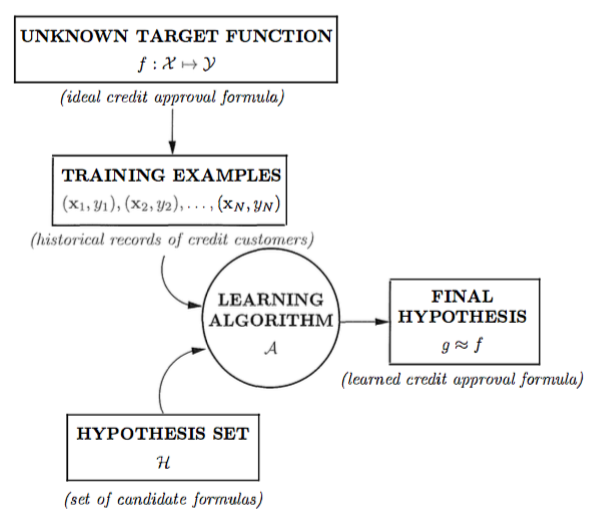
\includegraphics[width=0.7\textwidth]{include/dia.png}
            \end{figure}
    \end{frame}

    \begin{frame}[c]{Et kig på vores data?}
        \begin{columns}
            \begin{column}{0.6\textwidth}
                \vspace{-1.8em}
                \begin{block}{Input}
                    \begin{center}
                        \begin{tabular}{| c | r |}
                            \hline
                            Threshold                & 1           \\ \hline
                            Clump Thickness          & 7           \\ \hline
                            Uniformity of Cell Size  & 1           \\ \hline
                            Uniformity of Cell Shape & 4           \\ \hline
                            Epithelial Cell Size     & 2           \\ \hline
                            Bare Nuclei              & 3           \\ \hline
                            Bland Chromatin          & 8           \\ \hline
                            Normal Nucleoli          & 10          \\ \hline
                            Mitoses                  & 3           \\ \hline
                        \end{tabular}
                    \end{center}
                \end{block}
                \vspace{-1.2em}
                \begin{block}{Output}
                    \centering Ondartet eller godartet
                \end{block}
            \end{column}
            \pause

            \begin{column}{0.08\textwidth}
                \vspace{4em}
                \begin{Huge}
                    $$
                        \rightarrow
                    $$
                \end{Huge}
            \end{column}
            \begin{column}{0.3\textwidth}
                \vspace{-1.8em}
                \begin{block}{Data vektor}
                    $$
                        \left(
                        \begin{tabular}{c}
                            1      \\
                            7      \\
                            1      \\
                            4      \\
                            2      \\
                            3      \\
                            8      \\
                            10     \\
                            3
                        \end{tabular}
                        \right)
                    $$
                \end{block}
                \vspace{-0.9em}
                \begin{block}{Output}
                    \centering \alert{1}
                \end{block}
            \end{column}
        \end{columns}
    \end{frame}


\section{Perceptron algoritmen}
    \begin{frame}[t]{Valget af lærings-algoritmen}
        \begin{block}{Perceptron}
            Den laver et \emph{hyperplan} der adskiller data'en og finder en
            opdeling der giver en \alert{lav fejl}. \\
            \pause
            Tænk på den som en form for lineær regression på steroider
            $$
                y = ax + b
            $$
        \end{block}
        \pause
        \begin{block}{Eksempel på algoritmen}
            \vspace{-1em}
            \begin{figure}[h!]
                \centering
                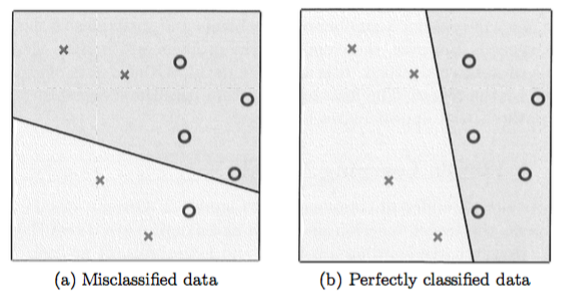
\includegraphics[width=0.5\textwidth]{include/per1.png}
            \end{figure}
        \end{block}
    \end{frame}


    \begin{frame}[t]{Algoritmen i ord}
        \begin{block}{Hvordan virker den?}
            Vi har en masse vektorer $x_1,x_2,\dots,x_n$ og en liste af svar
            $y_1,y_2,\dots,y_n$. \\
            \pause
            Vi lader $w$ være vores ``hjerne-vektor''. \pause
            \vspace{-1em}
            \begin{flalign*}
                \text{Godartet svulst : } \sum_{i=1}^d w_i x_i &> b \\
                \text{Ondartet svulst : } \sum_{i=1}^d w_i x_i &< b
            \end{flalign*}
            \pause
            \vspace{-1em}
            Vores hypotese bliver så
            $$
                h(x) = fortegn\left(\sum_{i=0}^d w_i x_i \right) = w \cdot x
            $$
            \pause
            \centering \alert{Men hvordan bestemmer vi $w$?}
        \end{block}
    \end{frame}

    \begin{frame}[c]{Hvordan den lærer}
        \begin{block}{Hvordan $w$ bestemmes}
            $$w = \text{ vælg tilfældige tal}$$
            \pause
            Vi forbedrer $w$ hver gang\\ \pause
            Hvis $x'$ er på den forkerte side af $w$ så lærer den ``erfaringen''
            ved formlen \pause
            $$
                w_{ny} = w + y' x'
            $$
            \pause
            Forsæt med at forbedre så længe så muligt.
        \end{block}
    \end{frame}


    \begin{frame}[plain]{Perceptron algoritme}
        \begin{block}{Pseduocode}
        \vspace{-1em}
        \begin{algorithm}[H]
            \begin{algorithmic}
                \State w = Tilfældige tal
                \State isLearning = True
                \While{isLearning}
                \State $isLearning = False$
                \For{$(x_i,y_i)$ in $X$}
                    \If{$sign(w^Tx_i) \neq y_i$ }
                        \State isLearning = True
                        \State $w = w + y_i x_i$
                    \EndIf
                \EndFor
                \EndWhile \\
                \Return w
            \end{algorithmic}
        \end{algorithm}
        \end{block}
    \end{frame}

\section{iPython og øvelser}
    \begin{frame}[t]{Øvelser}
        \begin{block}{iPython}
            Online python fortokler, med mulighed for nemt og hurtigt at lave
            opgaver til studerende. \\

            Gå ind på ``rotendahl.dk/vejle''
                \pause
                Redder vi så nogle liv?
                \pause
                Lad os kode det og se hvor god den er!
            \end{block}
    \end{frame}

    \begin{frame}[t]{Afslutning}
    \begin{block}{Hvor god er den? }
        I opgaverne kigger i kun på \alert{25 eksempler!} og tester på 75
        patienter \\
        \pause
        I kan forvente at den har ret på cirka $60-70\%$ af patienterne!.\\
        \pause
        Kører man den istedet med 500 eksempler og tester på 180. \pause
        Rammer den rigtigt 181 gange og forkert 2 gange. Det betyder at den
        har en succes rate på \alert{$98,9\%$!}
    \end{block}
    \pause
    \centering Spørgsmål?\\
    \end{frame}
\end{document}
